\documentclass{article}

\usepackage{amsmath,amssymb,amsthm}
\usepackage{tikz}
\usepackage[margin=2.0cm]{geometry}
\usepackage{float}

\newtheorem{proposition}{Proposition}

\author{Jacob Thomas Errington (260636023)\\Kelley Zhao (260573260)}
\title{Assignment \#1\\Distributed Systems -- COMP 512}
\date{20 October 2015}

\newcommand{\ms}{\text{ ms}}

\begin{document}

\maketitle

\section{Minis}

\begin{enumerate}
    \item
        In an asynchronous system, a process $p$ requests the time from a time
        server $S$, with a measured round-trip time of $24\ms$, and $p$
        receives $t = 10:54:23:674$ from $S$.

        \begin{enumerate}
            \item
                $p$ would set it's local clock to the received time, plus half
                the round-trip time, i.e.
                $$
                ps
                = t + \frac{T_\text{round}}{2}
                = 10 : 54 : 23 : 674 + 0 : 0 : 0 : 12
                = 10 : 54 : 23 : 686
                $$

            \item
                If $p$'s local time upon receipt of the response from $S$ is
                $ps = 10 : 54 : 24 : 005$, then setting its time to the value
                calculated above would result in a ``jump back in time''. This
                violates the expected monotonicity of the system clock. To
                remedy this, the system can run it's local clock more slowly
                for some time, to have it eventually become synchronized with
                the received time.
        \end{enumerate}

    \item
        There are many ways to marshal program data into a form suitable
        for transmission: XML (similarly JSON), Java's serialization, and
        Google Protocol Buffer, as well as others. For each of these three
        methods, here is an advantage it has over the other two.

        \begin{enumerate}
            \item
                XML and JSON have the advantage of being human-readable,
                text formats; if data is inspected while in transit, it can
                be understood without any additional tooling by a
                developer.

            \item
                Java's built-in serialization has the advantage of being
                extremely easy to use, from a developer's point of view.
                No additional libraries are required, since the
                functionality is built directly into the base Java Runtime
                Environment.

            \item
                Google Protocol Buffer is a binary format, like Java's
                built-in serialization, but is not tied to Java, so it can
                be used to interact with non-Java environments. It is also
                much faster than XML.
        \end{enumerate}

    \item
        Figures \ref{fig:lamporttimestamp} and \ref{fig:vectortimestamp} are
        timestamped diagrams of the communications between three processes. The
        first diagram uses a Lamport clock, whereas the second diagram uses a
        vector clock.

        \begin{figure}[ht]
            \centering

            \begin{tikzpicture}
                [
                    ->,
                    shorten >=1pt,
                    auto,
                    node distance=3.0cm,
                    semithick,
                    event/.style={shape=circle, fill=gray},
                    event delayed/.style={event, node distance=3.5cm},
                    timeline/.style={color=blue!70, very thin, -},
                    time endpoint/.style={node distance=16cm},
                    msg send/.style={node distance=2.0cm},
                    msg recv/.style={node distance=2.0cm},
                    msg send slow/.style={node distance=4.0cm},
                    msg recv slow/.style={node distance=4.0cm},
                    msg send very slow/.style={node distance=6.0cm},
                    msg recv very slow/.style={node distance=6.0cm}
                ]
                \node (p1)                                    {$p_1$};
                \node (p2) [below of=p1, node distance=2.5cm] {$p_2$};
                \node (p3) [below of=p2, node distance=2.5cm] {$p_3$};

                \node (end p1)
                      [right of=p1, time endpoint]
                      {};
                \node (end p2)
                      [right of=p2, time endpoint]
                      {};
                \node (end p3)
                      [right of=p3, time endpoint]
                      {};


                \path
                (p1) edge [timeline] node {} (end p1)
                (p2) edge [timeline] node {} (end p2)
                (p3) edge [timeline] node {} (end p3)
                ;

                \node (event p1 1)
                      [event, right of=p1, label=90:$1$]
                      {};

                \node (event p2 1)
                      [event, right of=p2, event delayed, label=90:$1$]
                      {};

                \node (event p1 2)
                      [event, right of=event p1 1, label=90:$3$]
                      {};

                \node (m1 send)
                      [msg send, right of=event p1 1, label=90:$2$]
                      {};

                \node (m1 recv)
                      [msg recv, right of=event p2 1, label=270:$3$]
                      {};

                \node (m2 send)
                      [msg send, right of=m1 recv, label=90:$4$]
                      {};

                \node (m2 recv)
                      [msg recv, right of=p3, node distance=8cm, label=270:$5$]
                      {};

                \node (m3 send)
                      [msg send, right of=m2 send, label=90:$5$]
                      {};

                \node (m5 send)
                      [msg send, right of=event p1 2, label=90:$4$]
                      {};

                \node (m4 send)
                      [msg send, right of=m2 recv, label=270:$6$]
                      {};

                \node (m5 recv)
                      [msg recv slow, right of=m3 send, label=90:$6$]
                      {};

                \node (m4 recv)
                      [node distance=3.775cm, right of=m5 send, label=90:$7$]
                      {};

                \node (m3 recv)
                      [msg recv, right of=m4 recv, label=90:$8$]
                      {};

                \node (event p3 1)
                      [event, right of=m4 send, label=90:$7$]
                      {};

                \path
                (m1 send) edge            node {$m_1$} (m1 recv)
                (m2 send) edge            node {$m_2$} (m2 recv)
                (m3 send) edge [pos=0.20] node {$m_3$} (m3 recv)
                (m4 send) edge [pos=0.25] node {$m_4$} (m4 recv)
                (m5 send) edge [pos=0.20] node {$m_5$} (m5 recv)
                ;

            \end{tikzpicture}

            \caption{
                A time series diagram of three intercommunicating processes
                with events annotated with their Lamport timestamps.
            }

            \label{fig:lamporttimestamp}
        \end{figure}

        \begin{figure}[ht]
            \centering

            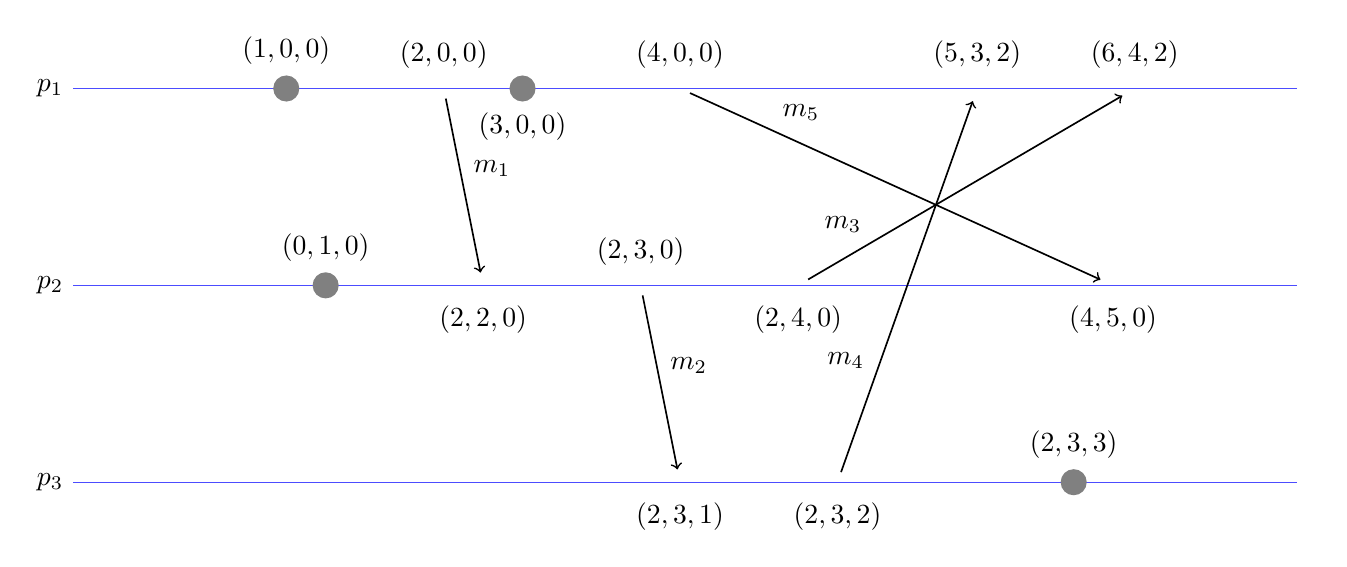
\begin{tikzpicture}
                [
                    ->,
                    shorten >=1pt,
                    auto,
                    node distance=3.0cm,
                    semithick,
                    event/.style={shape=circle, fill=gray},
                    event delayed/.style={event, node distance=3.5cm},
                    timeline/.style={color=blue!70, very thin, -},
                    time endpoint/.style={node distance=16cm},
                    msg send/.style={node distance=2.0cm},
                    msg recv/.style={node distance=2.0cm},
                    msg send slow/.style={node distance=4.0cm},
                    msg recv slow/.style={node distance=4.0cm},
                    msg send very slow/.style={node distance=6.0cm},
                    msg recv very slow/.style={node distance=6.0cm}
                ]
                \node (p1)                                    {$p_1$};
                \node (p2) [below of=p1, node distance=2.5cm] {$p_2$};
                \node (p3) [below of=p2, node distance=2.5cm] {$p_3$};

                \node (end p1)
                      [right of=p1, time endpoint]
                      {};
                \node (end p2)
                      [right of=p2, time endpoint]
                      {};
                \node (end p3)
                      [right of=p3, time endpoint]
                      {};


                \path
                (p1) edge [timeline] node {} (end p1)
                (p2) edge [timeline] node {} (end p2)
                (p3) edge [timeline] node {} (end p3)
                ;

                \node (event p1 1)
                    [event, right of=p1, label=90:{$(1,0,0)$}]
                    {};

                \node (event p2 1)
                    [event, right of=p2, event delayed, label=90:{$(0,1,0)$}]
                    {};

                \node (event p1 2)
                    [event, right of=event p1 1, label=270:{$(3,0,0)$}]
                    {};

                \node (m1 send)
                    [msg send, right of=event p1 1, label=90:{$(2,0,0)$}]
                    {};

                \node (m1 recv)
                    [msg recv, right of=event p2 1, label=270:{$(2,2,0)$}]
                    {};

                \node (m2 send)
                    [msg send, right of=m1 recv, label=90:{$(2,3,0)$}]
                    {};

                \node (m2 recv)
                    [msg recv, right of=p3, node distance=8cm,
                        label=270:{$(2,3,1)$}]
                    {};

                \node (m3 send)
                    [msg send, right of=m2 send, label=270:{$(2,4,0)$}]
                    {};

                \node (m5 send)
                    [msg send, right of=event p1 2, label=90:{$(4,0,0)$}]
                    {};

                \node (m4 send)
                    [msg send, right of=m2 recv, label=270:{$(2,3,2)$}]
                    {};

                \node (m5 recv)
                    [msg recv slow, right of=m3 send, label=270:{$(4,5,0)$}]
                    {};

                \node (m4 recv)
                    [node distance=3.775cm, right of=m5 send,
                        label=90:{$(5,3,2)$}]
                    {};

                \node (m3 recv)
                    [msg recv, right of=m4 recv, label=90:{$(6,4,2)$}]
                    {};

                \node (event p3 1)
                    [event, right of=m4 send, label=90:{$(2,3,3)$}]
                    {};

                \path
                (m1 send) edge            node {$m_1$} (m1 recv)
                (m2 send) edge            node {$m_2$} (m2 recv)
                (m3 send) edge [pos=0.20] node {$m_3$} (m3 recv)
                (m4 send) edge [pos=0.25] node {$m_4$} (m4 recv)
                (m5 send) edge [pos=0.20] node {$m_5$} (m5 recv)
                ;

            \end{tikzpicture}

            \caption{
                A time series diagram of three intercommunicating processes
                with events annotated with their vector clock timestamps.
            }

            \label{fig:vectortimestamp}
        \end{figure}
\end{enumerate}

\section{Eventual consistency}

Our algorithm to guarantee eventual consistency uses a vector clock to
timestamp the data $x_i$ held by process $p_i$ whenever a write occurs. Let
$v_i$ be a variable held locally by each process $i$ representing the last
write time to the data $x_i$ according to the vector clock. Each process $p_i$
also stores $k_i$ which is the process identifier of the \emph{originator} of
the write. When processes interact, they will exchange their data along with
the their metadata, i.e. its last write time and its originator identifier.

Suppose processes $i$ and $j$ exchange information and $k_i < k_j$. There are
three possibilities for how to handle the data.

\begin{enumerate}
    \item If $v_i < v_j$, then $p_j$ will accept $x_i$, overwriting its data
        $x_j$, and it will update $v_j$ to $v_i$. Process $p_j$ will also set
        $k_j := k_i$.

    \item If $v_i > v_j$, then $p_j$ will reject $x_i$, keeping its data as is.

    \item If $v_i$ cannot be compared with $v_j$, then the data writes happened
        concurrently. We must then examine the originators of the writes. Since
        $k_i < k_j$, $p_j$ will accept the data of $p_i$, setting $x_j := x_i$,
        $v_j := v_i$, and $k_j := k_i$.
\end{enumerate}

When writes occur locally in a process $p_i$, the timestamp is updated and the
originator is set $k_i := i$.

Using the concept of originators in this way allows processes with higher
identifiers to retransmit the data of processes with lower identifiers should
timestamps be incomparable in future exchanges, provided that local writes do
not occur in between the receipt of data and the retransmission. This will be
essential to the eventual consistency of the system.

\begin{proposition}
    Such a system is eventually consistent using the above communications
    algorithm.
\end{proposition}

\begin{proof}
    Consider the ordering on data items $x_i \sqsubseteq x_j$ defined by the
    following.
    $$
    x_i \sqsubseteq x_j
    \text{ if }
    v_i > v_j \lor (v_i \nless v_j \land k_i < k_j)
    $$

    It precisely captures the notion of comparing first based on time and if
    doing so is impossible, then comparing based on originator. Indeed, our
    algorithm uses this linear ordering to choose whether to accept or reject
    updates.

    Some process $p_i$ has the most recent data $x_i$ according to this
    relation. And given sufficient time, it will have communicated with every
    other process $p_j$, either directly or indirectly via originator metadata,
    causing $p_j$ to install $x_i$ on top of its own data.
\end{proof}

\section{Performance evaluation}

\begin{enumerate}
    \item
        In figure 1(a), RMI I appears to outperform RMI II in all types of
        serialization. In the case of bulk serialization, this difference is
        less important, probably because most of the serialization time is just
        spent copying the data array, so the overhead due to the different
        serialization strategies is less represented. In the other cases, the
        serialization overheads are more obvious: in the case of embedded
        objects especially, we see that as the complexity of the embedded
        objects increases, the time required by RMI II increases much more than
        the time required by RMI I.

        The most likely cause for this in my opinion is that RMI II includes a
        lot of metadata in the serialized form; including this data simply
        requires more time.

    \item
        In figure 1(b), we see that overall, HTTP is slower than raw TCP, as
        one would expect since it adds an extra layer. RMI I is tremendously
        slower than RMI II for this test, which involves fifty thousand calls.
        In the case of RMI I, that means fifty thousand new connections; the
        overhead of establishing TCP connections is certainly to blame for the
        major difference in time used by the RMI methods over HTTP. Over raw
        TCP, the difference is less pronounced, since both methods reuse
        sockets. Indeed, RMI I outperforms RMI II when using TCP.

        Those observations further support my idea that RMI II is including
        more metadata. More metadata means bigger messages, which could explain
        the difference seen in the case of messages sent over TCP in this
        figure.

    \item
        In figure 1(c), the size of the payload of the test is much larger and
        the number of messages sent is smaller, so the overheads are less
        important. Both RMI methods have similar time elapsed when transported
        over raw TCP.

        This puts the observation in the TCP half figure 1(b) into perspective.
        It suggests that RMI II uses some application-level handshaking that is
        creating a lot of overhead over the fifty thousand calls made in test
        1, whereas in test 2, the overhead of these handshakes is less
        important since there are only ten calls. Hence, both methods spend all
        their time simply copying the data array into the socket buffers.

        As for the HTTP part of figure 1(c), RMI II outperforms RMI I. It
        remains likely that the reason for this is the overhead incurred by
        creating new sockets for each HTTP request in RMI I. Indeed, over fifty
        thousand calls, this resulted in a major difference in elapsed time.
        Now over just ten calls, that difference ought to still be quite
        noticeable.

    \item
        In figure 1(d), we first observe that for each RMI type, the TCP
        version outperforms the HTTP version. In the case of RMI I, this is
        especially obvious, and like due to the connection reuse in its TCP
        variant. On the other hand, in the case of RMI II, the difference
        appears practically negligeable.

        As the complexity of the embedded objects grows, the elapsed time for
        RMI II grows faster than the elapsed time for RMI I; this is likely due
        to the serialization times as discussed before.

        It is curious that the HTTP variant of RMI I is faster than the HTTP
        variant of RMI II, however. I believe that this occurs because the
        serialization overhead in RMI II outweighs the penalty incurred on RMI
        I by having to open new sockets for each invocation.
\end{enumerate}

\end{document}
